\documentclass[]{foi} 
\usepackage[utf8]{inputenc}
\usepackage{lipsum}
\addbibresource{lib.bib}

\vrstaRada{\projekt}

\title{Aplikacija za preporuke}
\predmet{\predmetTBP}

\author{Hrvoje Lesar} 
\spolStudenta{\musko} 

\mentor{Bogdan Okreša Đurić}
\spolMentora{\musko} 
\titulaProfesora{dr. sc.}

\godina{2024}
\mjesec{Siječanj}

\indeks{0016133479}

\smjer{Organizacija poslovnih sustava}

% \kljucneRijeci{riječ; riječ; ...riječ; Obuhvaća $7\pm2$ ključna pojma koji su glavni predmet rasprave u radu.}
% keywords including 7 +/- 2 syntagms

\acrodef{VAS}{višeagentni sustav}


\begin{document}

\maketitle

\tableofcontents

\makeatletter \def\@dotsep{4.5} \makeatother
\pagestyle{plain}

\chapter{Uvod}

Kroz projekt će biti teoretski obrađene polustrukturirane baze podataka, polustrukturirani podaci, jedna od 
često korištenih polustrukturiranih baza podataka MongoDB i teoretske osnove sustava za preporuke.

Cilj rada je implementirati aplikaciju za preporuke knjiga. Ovaj cilj će se postići korištenjem programskog
jezika \texttt{Go} u kojemu će se izrađivati web aplikacija. Aplikacija mora imati mogućnost komunikacije
s bazom podataka MongoDB i način za postavljanje upita. Odabran je programski jezik \texttt{Go} zbog relativne
jednostavnosti jezika i mogućnosti brze iteracije i izrade aplikacija, također ima vrlo dobru podršku za web.

Web aplikacija mora imati mogućnost prikaza preporuka određenom korisniku. Preporuka se mora generirati na temelju
drugih korisnika te se preporuke moraju mijenjati u slučaju promjene "ukusa" korisnika tj. korisnik i drugi
korisnici imaju značaj i utjecaj na preporuke.

\chapter{Polustrukturirane baze podataka}

\section{Polustrukturirani podaci}

Glavna ideja polustrukturiranih podataka je predstavljanje podataka kao vrstu strukture koja ima nalik na graf ili stablo.
Iako su dopušteni ciklusi između vrhova grafa, općenito takvu vrstu grafa možemo nazivati stablima \cite{buneman1997semistructured}.
Na slici \ref{fig:primjer_polustrukturiranih_podataka} je prikazan primjer modela podataka formaliziran u strukturu grafa.
Bridovi grafa su označeni tipom podatka ili više apstraktnim tipom koji se dalje grana. Prolaskom kroz graf moguće je
primijetiti da postoje dva različita načina prema kojima je opisan film. U prvom su glumci, filmska ekipa direktno nabrojeni,
dok u drugom postoji grananje na glumce i kreditirane glumce. Zadnja grana grafa opisuje TV seriju koja opet ima drugačiju
strukturu u usporedbi s strukturom filmova.

\begin{figure}[h!]
	\centering
	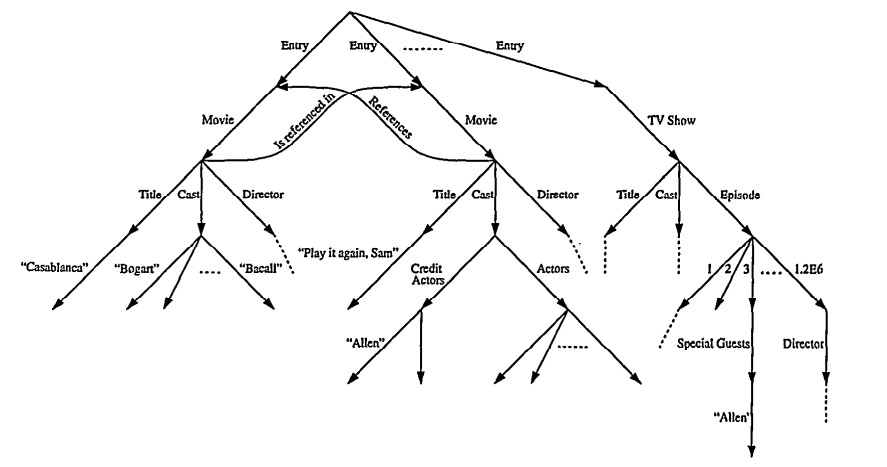
\includegraphics[width=0.9\textwidth]{slike/graf_primjer.png}
	\caption{Primjer polustrukturiranih podataka u obliku grafa \cite{buneman1997semistructured}}
	\label{fig:primjer_polustrukturiranih_podataka}
\end{figure}

Polustrukturirani podaci su organizirani u semantičke entitete, ali nisu striktno u skladu s formalno strukturiranim strogim tipovima podataka.
Konceptualni model polustrukturiranih podataka mora sadržavati nekoliko svojstava kao što su reprezentacija nepravilnih i heterogenih struktura
kao prikazanih na slici \ref{fig:primjer_polustrukturiranih_podataka}, hijerarhijske odnose uz nehijerarhijske vrste odnosa, kardinalnost,
relacije n-niza, poredak i reprezentaciju mješovitog sadržaja \cite{ganguly2012evaluations}.

\section{Vrste polustrukturiranih baza podataka}

Polustrukturirane baze podataka možemo podijeliti na četiri glavne vrste \cite{abramova2013nosql}:

\begin{enumerate}
	\item Key-Value store (Pohrana ključeva i vrijednosti); Podaci se pohranjuju kao skup ključeva i vrijednosti.
	      Ključevi su jedinstveni te se pristupa podacima povezivanjem ključa s vrijednosti.
	      Vrijednosti ne moraju striktno biti informacije, mogu biti drugi ključevi.
	\item Baze podataka temeljene na dokumentima; Mogu se definirati kao setovi ključeva i vrijednosti.
	      Svaki dokument je identificiran unikatnim ključem. Tip dokumenta je definiran prema znanim standardima
	      koji su većini slučajeva XML ili JSON. Pristup podacima moguć je korištenjem ključa ili određenih vrijednosti.
	\item Column-family (Obitelj stupaca); Podaci su postavljeni u stupce tj. sama struktura podataka i organizacija podatak
	      se sastoji od stupaca super-stupaca, i obitelji stupaca. Struktura baze je definirana kroz super-stupce i obitelj stupca.
	      Novi stupci se mogu dodavati po potrebi. Pristup podacima je moguć naznačujući obitelj stupca, ključ, stupac što će
	      rezultirati dohvaćanjem vrijednosti.
	\item Graf baze podataka; Ova vrsta se koristi kad se podaci mogu prikazati kao graf, jedan primjer su društvene mreže
	      i veze između različitih korisnika.
\end{enumerate}

\section{MongoDB}

MongoDB je polustrukturirana baza temeljena na dokumentima. Dokumenti su grupirani u kolekcije prema njihovoj strukturi.
Dopušteno je spremanje dokumenta različitih struktura, no zbog boljih performansi preporuka je grupirati dokumente s
istom ili sličnom strukturom \cite{abramova2013nosql}. MongoDB koristi BSON kao format za spremanje dokumenata. BSON je kratica za Binary JSON.

Svaki novi dokument je moguće identificirati poljem \_id, te je za svaku kolekciju automatski kreiran indeks preko \_id polja.
Neke od najbitnijih karakteristika MongoDB-a su trajnost i moguće paralelno čitanje i pisanje podataka.
Trajnost je omogućeno kroz kreiranje replika baze, MongoDB koristi master-slave (gospodar-rob) mehanizam za replikaciju.
Omogućava definiranje jednog gospodara i jednog ili više robova. Gospodar je jedina replika kojoj je dozvoljeno pisanje i čitanje
dok robovi služe samo kao sigurnosna kopija. U slučaju da se gospodar replika sruši, replika rob s najnovijim podacima je promovirana
u novog gospodara. Sve replike su asinkrone što znači da izvršena ažuriranja nisu odmah vidljiva na svim replikama.
MongoDB postiže paralelno čitanje i pisanje podataka zaključavanjem podataka. Podaci koji se trenutno ažuriraju su zaključani
kako nebi bili pročitani zastarjeli podaci ili kako se nebi dogodilo više upisa u isto vrijeme te više nebi bilo moguće
odrediti valjanost upisanih podataka.

\section{Sustavi za preporuke}

Sustavi za preporuke se koriste za izradu kolekcije stavaka koje bi mogle interesirati određene korisnike.
Dizajn sustava ovisi o domeni problema, proizvoda, stavaka koje se žele preporučiti te dostupnosti podataka i posebnih
karakteristika prema kojima bi bilo moguće kreirati preporuku \cite{melville2010recommender}.
Sustavi za preporuke se razlikuju po načinu na koji analiziraju izvor podataka kako bi odredili
srodnost između korisnika i stavka koje se mogu koristiti za identifikaciju podudarnih parova.

Načini pristupa rješavanju problema preporuka moguće je kategorizirati u nekoliko glavnih kategorija \cite{lu2012recommender}:
\begin{enumerate}
	\item Kolaborativno filtriranje; Kolaborativno filtriranje radi na principu prikupljanja povratnih informacija od korisnika.
	      Povratne informacije su uglavnom u obliku ocjena za stavke u određenoj domeni. Iskorištavanjem sličnosti u ponašanju
	      ocjenjivača se određuje manji broj korisnika kojima je moguće preporučiti neku stavku.
	\item Preporuke temeljene na sadržaju; Daju preporuke uspoređujući prikaze opisa sadržaja koji opisuju neku stavku s
	      prikazima sadržaja koji zanimaju korisnika.
	\item Hibridni pristupi; Pokušava kombinirati kolaborativno filtriranje i preporuke temeljene na sadržaju kako bi
	      preporuke bile što bolje i točnije.
\end{enumerate}

\chapter{Model baze podataka} \label{cha:model_baze_podataka}

\section{Korišteni skup podataka}

Skup podataka koji je korišten kao temeljni je \texttt{goodreads-10k} skup. Skup sadrži oko deset tisuća knjiga i oko šest milijuna ocjena
knjiga, tagove i žanrove dodijeljene knjigama od strane korisnika. Inicijalni skup je raspoređen u nekoliko \texttt{.csv} datoteka i može
se prikazati sljedećim dijagramom:

\begin{figure}[h!]
	\centering
	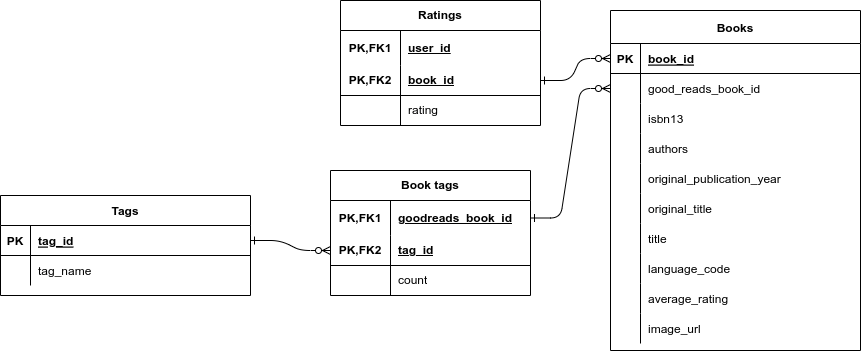
\includegraphics[width=0.9\textwidth]{slike/goodbooks-10k_dijagram.png}
	\caption{Dijagram strukture podataka korištenog skupa podataka}
	\label{fig:struktura_podataka}
\end{figure}

Kroz dijagram na slici \ref{fig:struktura_podataka} je vidljivo da su podaci strukturirani na način pogodan za relacijske baze podataka.
Korišteni skup će biti direktno importiran u MongoDB no potrebno će ga biti transformirati u skup više pogodan za rad s polustrukturiranim bazama.
Kolekcije kreirane importiranjem podataka imaju nazive \texttt{tags}, \texttt{ratings}, \texttt{book\_tags}, \texttt{books}.

\section{Pretvorba podataka}

Sve navedene naredbe moguće je pokrenuti preko mongo shella u bazi podataka koja ima importiran prije definiran skup podataka.
Pretvorba podataka započinje smanjivanjem dostupnih broja tagova, tj. korištenjem samo onih najpopularnijih. Pošto su tagovi iz izvornog
skupa podataka definirani od strane korisnika mogu imati vrlo različite nazive i imati različita značenja za korisnike, time bi
najpopularniji tagovi morali filtrirati one manje korisne.

\begin{minted}[samepage]{javascript}
db.book_tags.agreggate([
    { $group: { _id: "$tag_id", totalCount: { $sum: "$count", }, }, },
    { $sort: { totalCount: -1, }, },
    { $limit: 300, },
    { $lookup: { from: "tags", localField: "_id", foreignField: "tag_id", as: "tag", }, },
    { $group: { _id: "$tag", }, },
    { $unwind: "$_id", },
    { $replaceRoot: { newRoot: "$_id", }, },
    { $out: "most_popular_tags", },
])
\end{minted}
\captionof{listing}{Kreiranje najpopularnijih tagova}
\label{lst:tagovi}

Sljedeće se dodaju žanrovi knjigama (žanrovi su izvedeni iz tagova). Definirani upit prolazi kroz svaki tag,
provjerava koje knjige imaju dodijeljen trenutno selektirani tag, te ažurira sve dokumente u kolekciji \texttt{books}
sa tagom tj. žanrom koji pripada knjizi.

\begin{minted}[samepage]{javascript}
    db.most_popular_tags.find({}).map((tag) => {
        db.book_tags.agreggate([
            { $match: { tag_id: tag.tag_id } },
            { $project: { goodreads_book_id: 1 } }
        ]).map((tagIds) => {
            db.books.updateMany({goodreads_book_id: { $in: tagIds }}, { $addToSet: { genres: tag.name }})
        });
    })
\end{minted}
\captionof{listing}{Dodavanje žanrova knjigama}
\label{lst:zanrovi}

Zadnji korak agregiranje korisnika i njihovih ocjena knjiga u jednu kolekciju. U ovom koraku se svakom korisniku
dodjeljuje skup knjiga koje su ocijenili.

\begin{minted}[samepage]{javascript}
    db.ratings.agreggate([
        { $lookup: { from: "books", localField: "book_id", foreignField: "book_id", as: "book", }, },
        { $project: { _id: 1, user_id: "$user_id", rating: "$rating", book: { $arrayElemAt: ["$book", 0], }, }, },
        { $group: { _id: "$user_id", book_ratings: { $push: { rating: "$rating", book: "$book", }, }, }, },
        { $out: "users", },
    ])
\end{minted}
\captionof{listing}{Dodavanje žanrova knjigama}
\label{lst:korisnici}

Završne kolekcije u bazi se mogu reprezentirati kao što je prikazano na sljedećoj slici \ref{fig:izvedene_kolekcije}.
Vidljivo je da su napravljene tri kolekcije \texttt{books}, \texttt{users} i \texttt{most\_popular\_tags}.
Kolekcija \texttt{books} sadržava knjige i ima na novo dodano polje \texttt{genres} što je lista žanrova knjige.
Kolekcija \texttt{users} su korisnici, identificirani samo svojim id-om, te svaki korisnik ima listu knjiga koje je
ocijenio, svaki element liste je ocjena i cijeli zapis ocjenjene knjige.

\begin{figure}[h!]
	\centering
	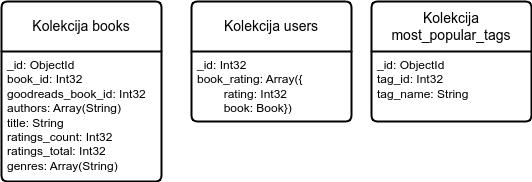
\includegraphics[width=0.9\textwidth]{slike/kolekcije.png}
	\caption{Izvedene kolekcije}
	\label{fig:izvedene_kolekcije}
\end{figure}


\section{Implementacija}

Sustav je implementiran u programskom jeziku \texttt{Go}. Za prikaz preporuka kreiran je web poslužitelj koji poslužuje web stranicu sa preporukama za
određenog korisnika. Konkretno se preporučuju knjige. Aplikacija za komunikacijom s MongoDB koristi Mongo Driver biblioteku.
Na web stranici postoji nekoliko vrsta preporuka:
\begin{itemize}
	\item preporuke temeljene na kolaborativnom filtriranju,
	\item preporuke određene prema najvišim ocjenama knjiga
	\item preporuke određene prema najvišim ocjenama knjiga prema određenom žanru
\end{itemize}
Korisnici imaju mogućnost dodavanja, izmjene, brisanja ocjena knjigama, time potencijalno mijenjanju preporuke za "slične" korisnike
i utječu na prosječnu ocjenu preporuka koje su određene prema najvišim ocjenama.

U nastavku svi implementirani MongoDB upiti će zbog lakšeg čitanja biti pretvoreni u upite koji se mogu izvršiti u \texttt{mongosh}.

\subsection{Najbolje ocjenjene knjige}

Jedan od načina na koji se preporučuju knjige je pronalaženje knjiga s najboljim ocjenama korisnika.
Za ovaj scenarij imamo dva slučajeva, preporuke knjiga koje imaju najbolje prosječne ocjene korisnika
i preporuke knjiga koje imaju najbolje prosječne ocjene korisnika u određenom žanru.

Upit koji se postavlja bazi podataka za dohvaćanje knjiga je sljedeći:
\begin{minted}[samepage]{javascript}
    db.users.agreggate([
        { $unwind: "$book_ratings" },
        { $group: { _id: "$book_ratings.book", totalRatings: { $sum: "$book_ratings.rating"}, count: { $sum: 1 } } },
        { $project: { _id: "$_id._id", book: "$_id", totalRating: 1, count: 1, averageRating: { $divide: ["$totalRating", "$count"] } } },
        { $sort: { averageRating: -1 } },
        { $project: { _id: "$_id._id", book: "$_id", totalRating: 1, count: 1, averageRating: { $round: ["$averageRating", 2] } } },
    ])
\end{minted}
\captionof{listing}{Upit za najbolje ocjenjene knjige}
\label{lst:najbolje_ocjene_knjiga}

Upit prolazi kroz kolekciju \texttt{users} te prvo za svakoga korisnika listu njihovih pretvara u jednu listu koja se nakon toga
grupira prema knjigama, izračunava se ukupna ocjena i broj danih ocjena. Zatim treći korak \texttt{project} prikazuje polja
objekta koja želimo prikazati i kreira prosječnu ocjenu za svaku knjigu. Knjige su sortirane silazno prema prosječnoj ocjeni
te se prosječna ocjena zaokružuje na dvije decimale.

\subsection{Kolaborativno filtriranje}

Kolaborativno filtriranje je implementirano kroz algoritam K-najbližih susjeda (KNN - k-nearest neighbours).
Prvo odabiremo korisnika za kojega želimo generirati preporuke potom radimo upit u bazu za sve korisnike koji nisu taj korisnik.
Za svakog korisnika određujemo vrijednost koja označava kako je sličan odabranom korisniku.
To se radi na način da ako korisnik ima ocjenjene knjige koje ima i odabrani korisnik dobiva brojčanu vrijednost ovisno o
sličnosti ocjena. Tako će korisnik koji ima jednake ocjene knjiga kao odabrani imati vrijednost \texttt{1.0} što bi označavalo
da su korisnici jednaki tj. pretpostavljamo da vole jednake knjige, dok vrijednost od \texttt{0.0} označava da se korisnici uopće
ne podudaraju. Poslije izračuna vrijednosti korisnici se sortiraju silazno prema izračunatim vrijednostima te se za preporuke
uzimaju knjige koje nisu ocjenjene od odabranog korisnika, a jesu među ocjenjenim knjigama najsličnijih.

\subsection{Dodavanje, brisanje, promjena ocjena}

Što se tiće dodavanja, brisanja i promjena ocjena koriste se sljedeći upiti:
\begin{minted}[samepage]{javascript}
    db.users.updateOne({ _id: userId }, { $push: { book_ratings: { rating: newRating, book: book } } })
\end{minted}
\captionof{listing}{Dodavanje ocjene knjizi}
\label{lst:dodavanje_ocjene_knjizi}

U isječku koda \ref{lst:dodavanje_ocjene_knjizi} \texttt{userId}, \texttt{newRating} i \texttt{book} su varijable koje
se prosljeđuju u upit. Sam upit za dodavanje pronalazi korisnika s vrijednošću \texttt{\_id} jednakom \texttt{userId} te u
listu \texttt{book\_ratings} dodaje knjigu i ocjenu.

\begin{minted}[samepage]{javascript}
    db.users.updateOne({ _id: userId }, { $set: { "book_ratings.$[x].rating": newRating } }, { arrayFilters: [ { "x.book.book_id": bookId } ] })
\end{minted}
\captionof{listing}{Promjena ocjene}
\label{lst:promjena_ocjene}

U isječku koda \ref{lst:promjena_ocjene} se koriste \texttt{arrayFilters} kako bi se odabrao i ažurirao točan zapis u listi ocjena.
Opcija \texttt{arrayFilters} postavlja \texttt{x} kao identifikator indeksa liste na kojemu se nalazi knjiga s \texttt{bookId} te se u
vrijeme pokretanja upita ažurira samo to polje liste.

Zadnji upit je brisanje ocjene. Brisanje se radi korištenjem \texttt{\$pull} naredbe koja će iz liste maknuti zapise koji zadovoljavaju zadane uvjete.
\begin{minted}[samepage]{javascript}
    db.users.updateOne({ _id: userId }, { $pull: { book_ratings: { "book.book_id": bookId } } } )
\end{minted}
\captionof{listing}{Promjena ocjene}
\label{lst:brisanje_ocjene}

\chapter{Primjeri korištenja}

Slika \ref{fig:najpopulranije_knjige} prikazuje neke od knjiga koje su dane kao preporuke prema najboljim ocjenama.
Ocjene knjiga su vidljive ispod naslova knjige i autora.

\begin{figure}[h!]
	\centering
	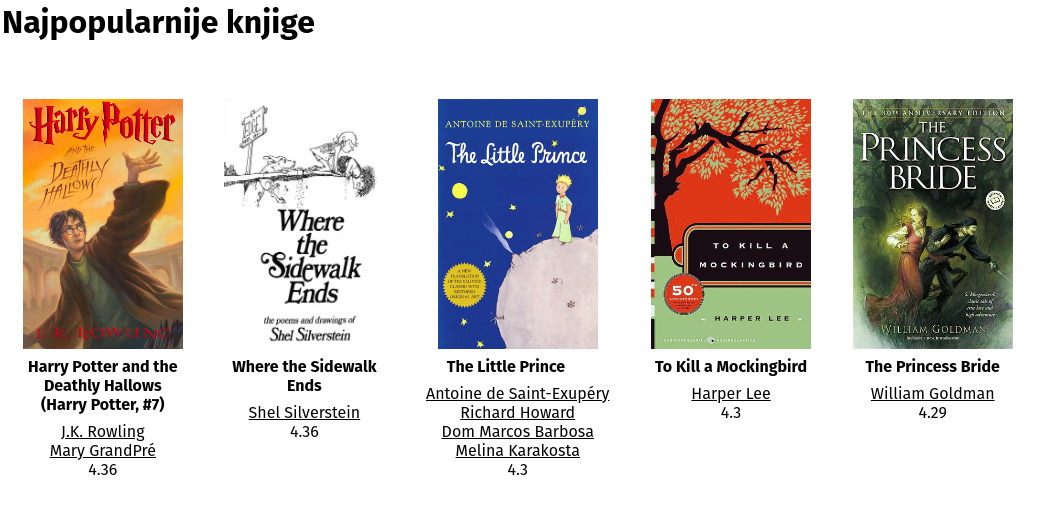
\includegraphics[width=0.9\textwidth]{slike/najpop.png}
	\caption{Najpopularnije knjige}
	\label{fig:najpopulranije_knjige}
\end{figure}

Slika \ref{fig:prema_tagu} prikazuje neke od knjiga koje su dane kao preporuke prema najboljim ocjenama uz odabrani tag tj. žanr.
Prikazane su samo knjige koje imaju dodijeljen odabrani žanr \texttt{high-fantasy}.

\begin{figure}[h!]
	\centering
	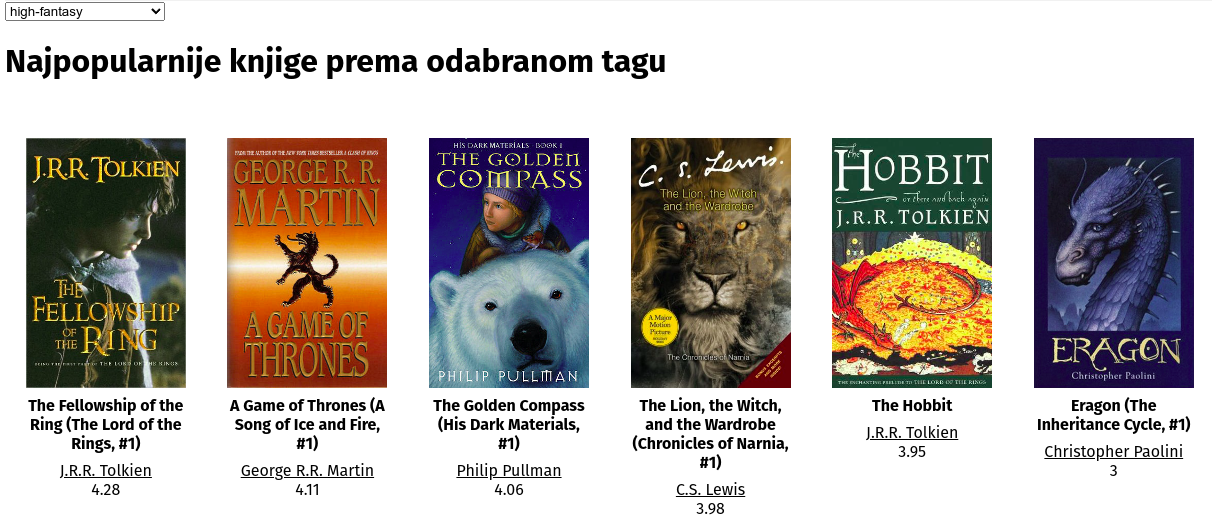
\includegraphics[width=0.9\textwidth]{slike/prema_tagu.png}
	\caption{Najpopularnije knjige prema odabranom tagu}
	\label{fig:prema_tagu}
\end{figure}

Slika \ref{fig:slicni} prikazuje korisnika koji ima najsličnije ocjene knjiga trenutnome.
Možemo primijetiti da oba korisnika imaju dane ocjene za knjige The Da Vinci Code, Memoirs of a Geisha i druge.
Neke od ocjena su također jednake što više pridonosi sličnosti korisnika. U zagradi pored Korisnik ID: 127 je zapisan
broj koji odgovara sličnosti između ova dva korisnika.
\pagebreak

\begin{figure}[h!]
	\centering
	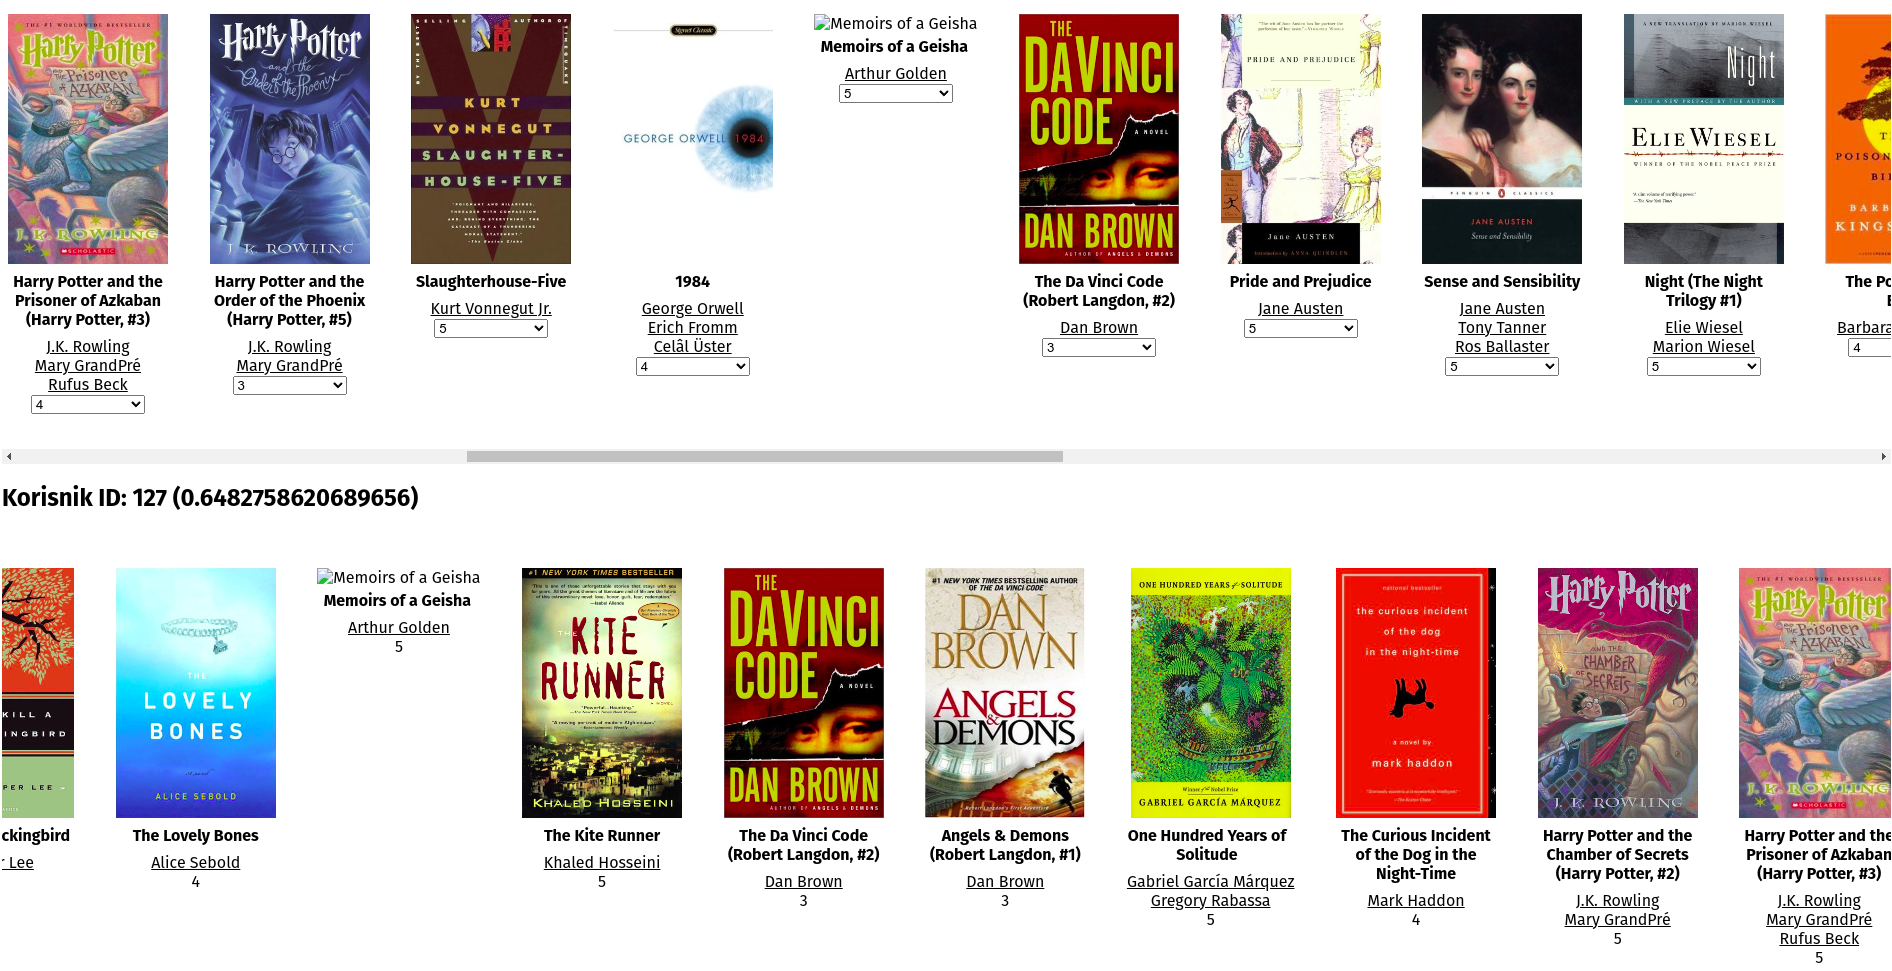
\includegraphics[width=0.9\textwidth]{slike/slicni_korisnik_15.png}
	\caption{Prikaz slicnog korisnika trenutnom odabranom}
	\label{fig:slicni}
\end{figure}

Slika \ref{fig:preporuke} prikazuje preporuke za odabranog korisnika na slici \ref{fig:slicni}.
Sve preporuke su uvijek knjige koje taj korisnik nije ocijenio i nalaze se u skupu knjiga koje su ocijenili
slični korisnici.

\begin{figure}[h!]
	\centering
	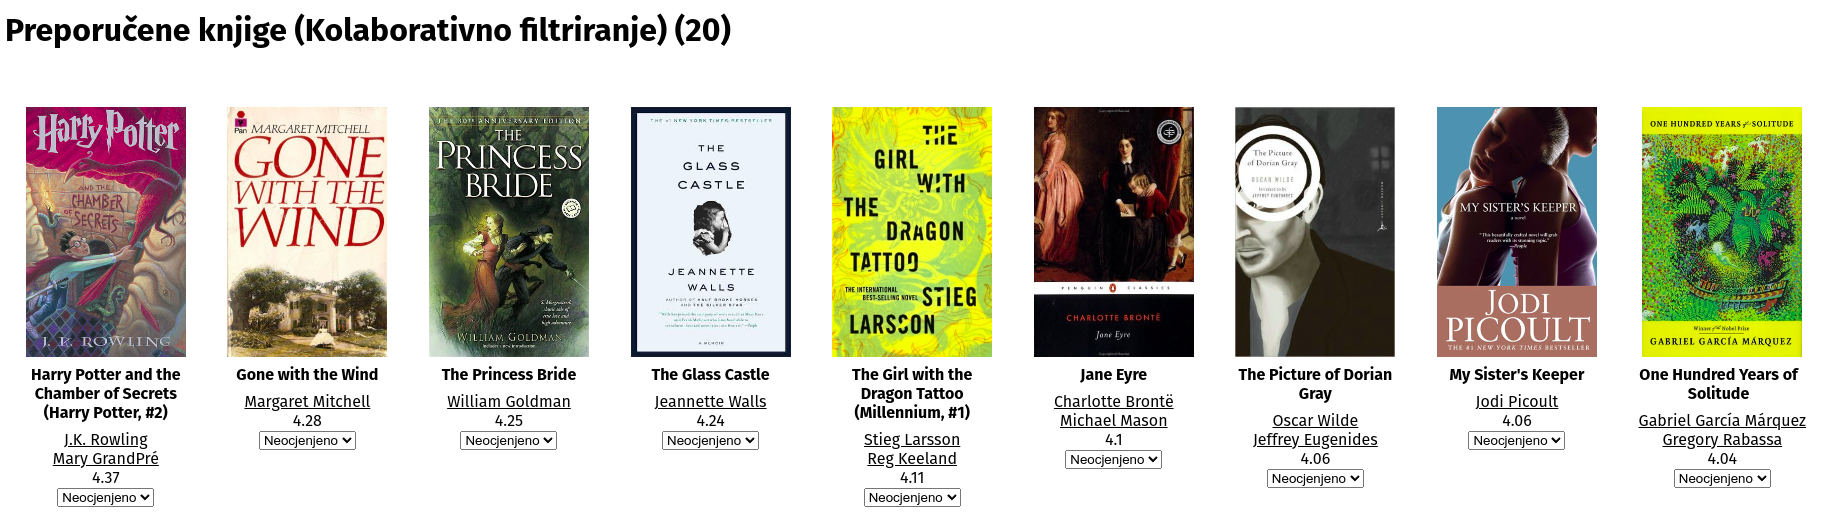
\includegraphics[width=0.9\textwidth]{slike/preporuke.png}
	\caption{Preporuke}
	\label{fig:preporuke}
\end{figure}

Slika \ref{fig:promjena_ocjene} sadrži prikaz načina promjene ocjene.

\begin{figure}[h!]
	\centering
	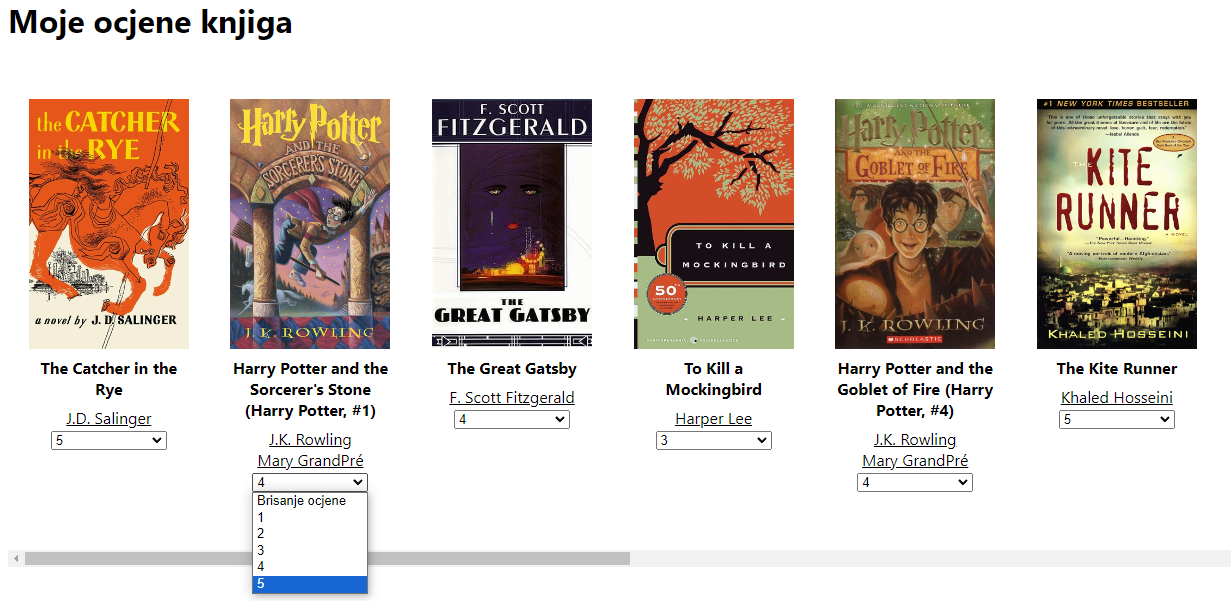
\includegraphics[width=0.9\textwidth]{slike/promjena_ocjene.png}
	\caption{Promjena, brisanje ocjene}
	\label{fig:promjena_ocjene}
\end{figure}

\chapter{Zaključak}

Kroz rad su prikazane osnovne ideje polustrukturiranih baza podataka, objašnjeni način na koji ovakve vrste baza podataka
pohranjuju podatke i struktura tih podataka.
Opisan je MongoDB korišten za pohranu podataka i pokretanje upita na podacima, te je navedena osnovna ideja sustava za preporuke,
različite vrste sustava i načina implementacija.

U poglavlju \ref{cha:model_baze_podataka} prikazana je struktura podataka koji se koriste za preporučivanje knjiga.
Opisan je proces pretvorbe podataka iz odabranog skupa podataka u polustrukturirane.
Za implementaciju aplikacije korišten je programski jezik \texttt{Go}. Odabran je zbog svoje relativne jednostavnosti i brzine
razvijanja aplikacija. Ima dobru podršku za komunikaciju s bazom MongoDB.
Implementirana je web aplikacija za preporuke knjiga.

Web aplikacija omogućuje korisnicima ocjenjivanje knjiga. Ovisno o ocjenama korisnika predlaže knjige koje su ocijenili
slični korisnici. Slične korisnike određuje koristeći algoritam K-najbližih susjeda. Svakom promjenom ocjena, ocjenjivanjem nove
knjige ili brisanjem ocjena korisnik će potencijalno dobiti nove preporuke.

\makebackmatter

\end{document}
